\section{Performance Characterization}

% Characterizations of each of our micro- and macro-benchmarks. We describe which drone applications require parallel computer architectures, which ones require computers with fast serial performance, and which ones would benefit from parallel architectures but run fast enough on serial computers.

We plot the performance breakdowns of our micro-benchmarks in Fig~\ref{fig:micro-perf}. We found that computer vision kernels such as \textit{object detection} achieve high performance only on computers with highly parallel  architectures such as the TX1. We found that SLAM micro-benchmarks require such-and-such architecture to achieve high performance. We found that the path-finding micro-benchmarks achieve high performance on all our processors, but they achieve even higher performance on computers with such-and-such architecture.

\begin{figure}[h]
\centering
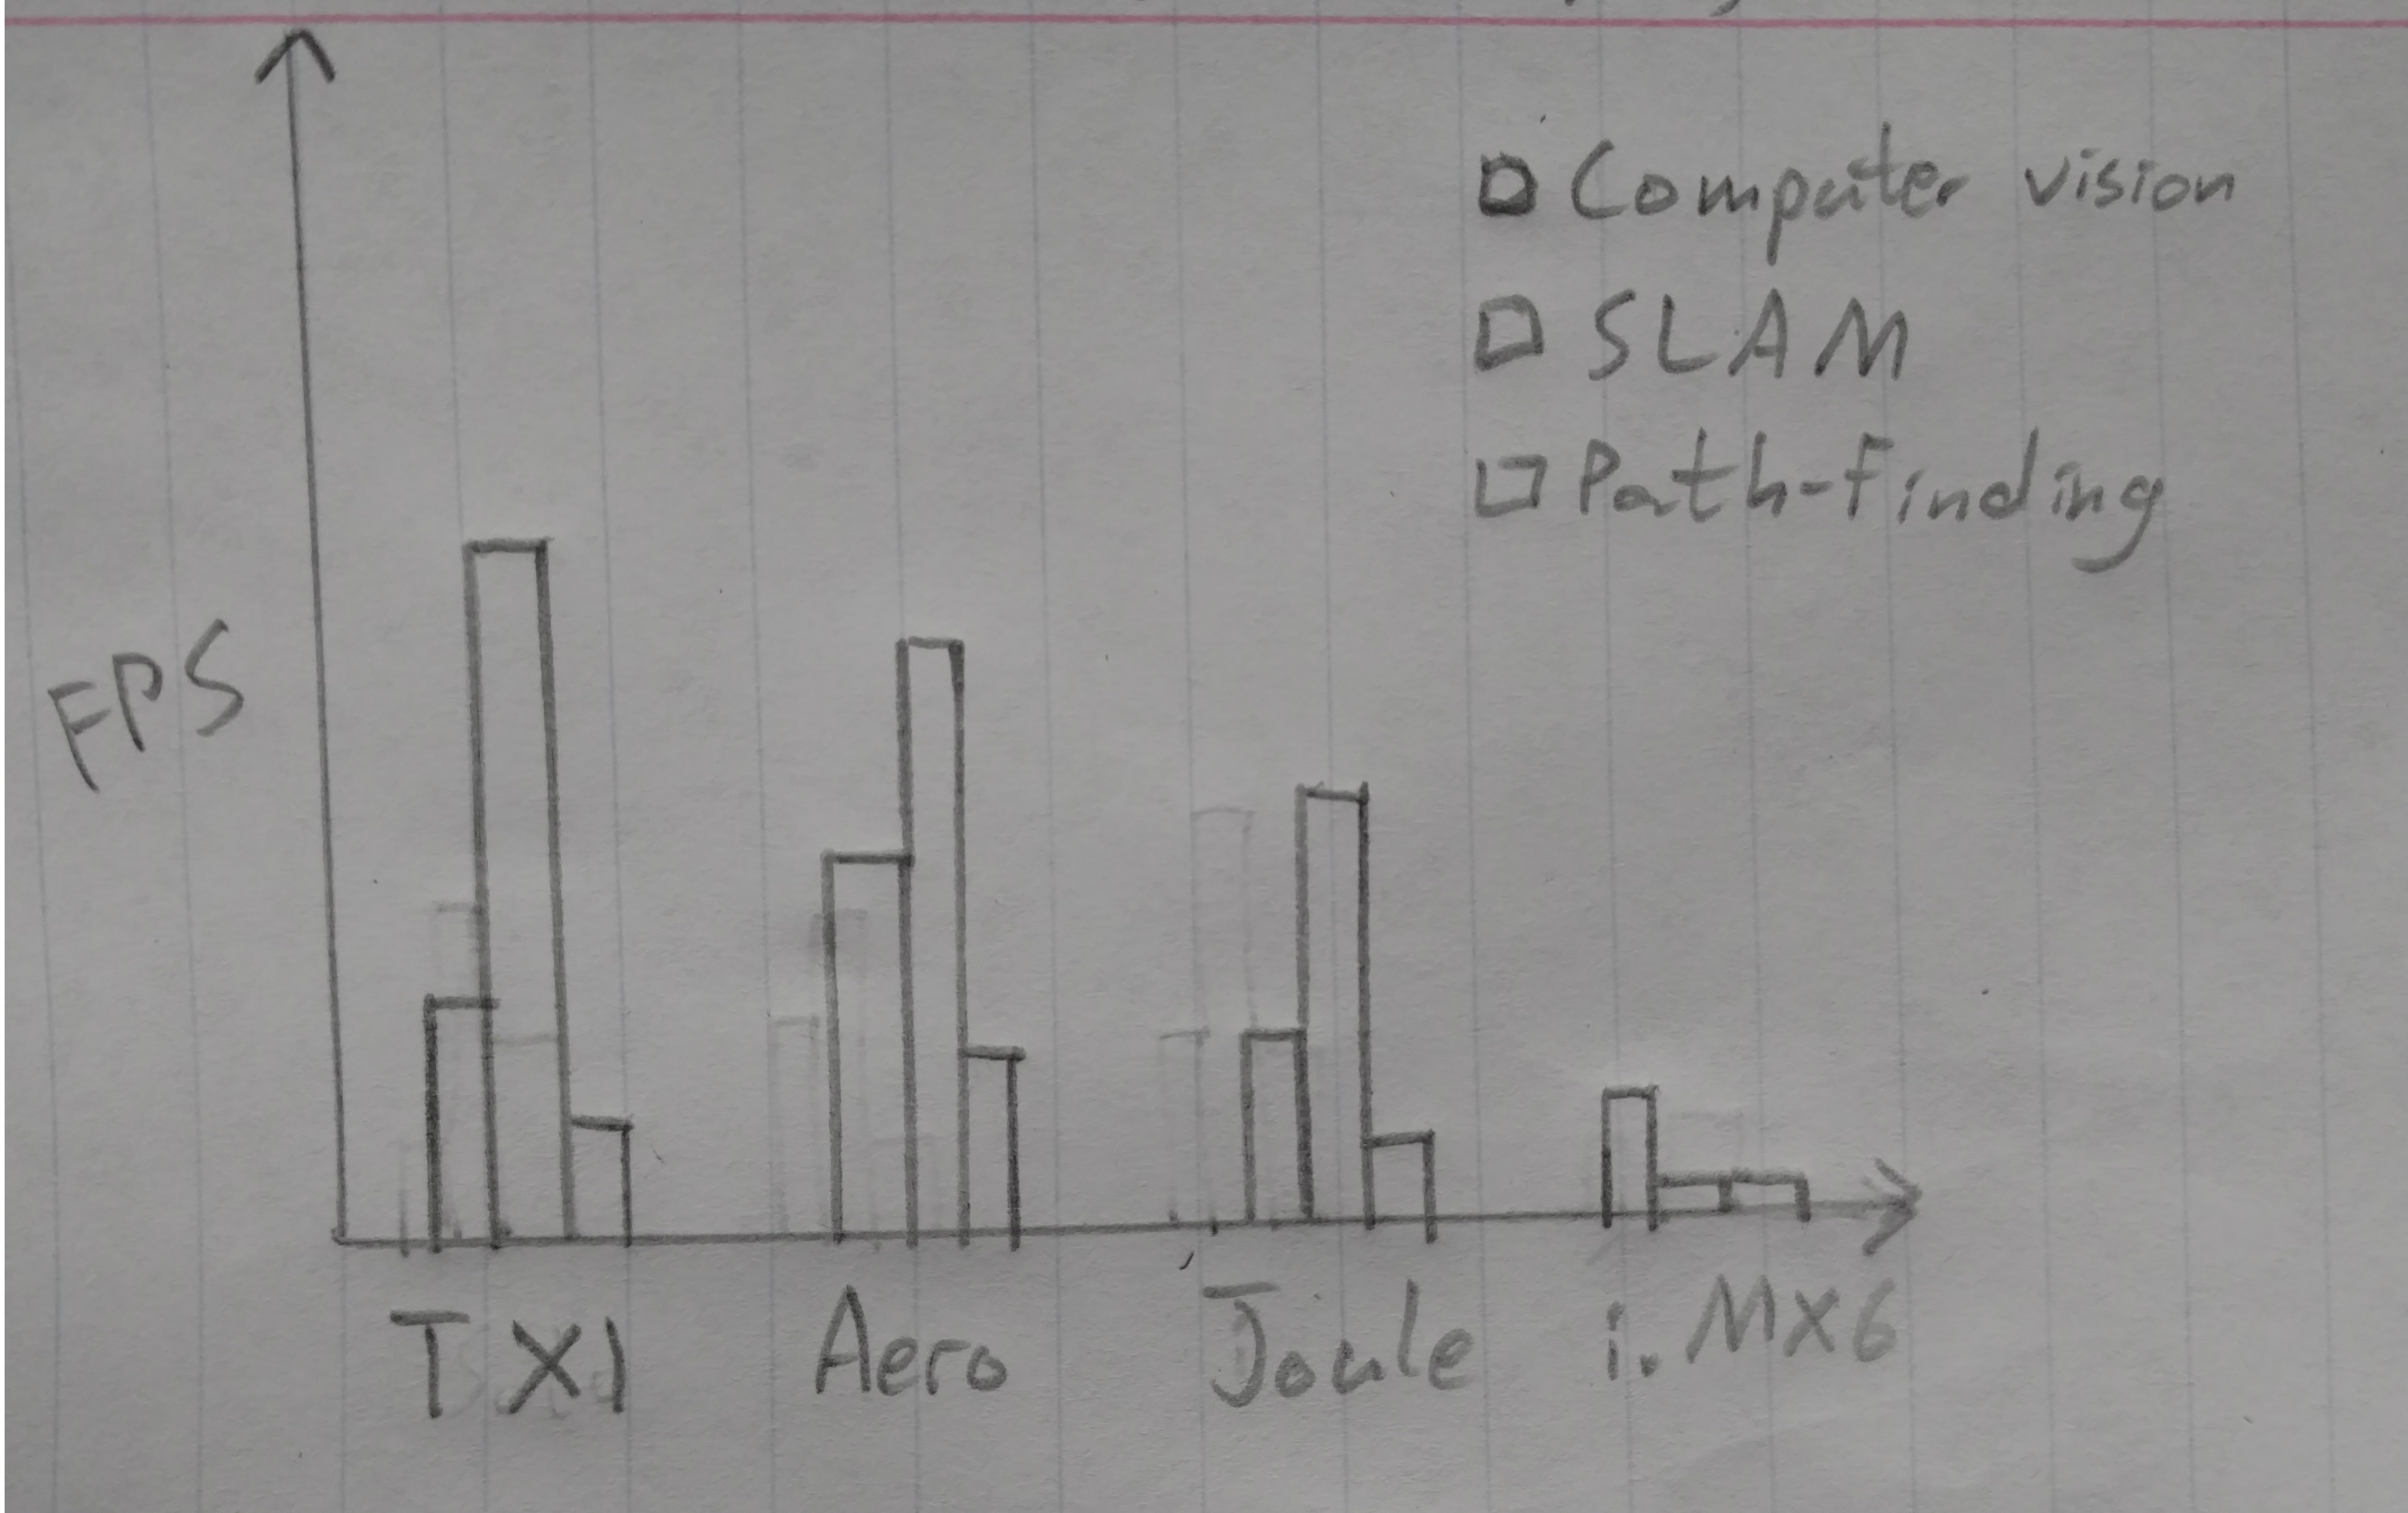
\includegraphics[width=\linewidth]{figs/micro-perf}
\caption{Performance of computational micro-benchmarks on various companion computers.}
\label{fig:micro-perf}
\end{figure}

We plot the performance breakdowns of our macro-benchmarks when running in simulated environments designed for AirSim, as seen in Fig.~\ref{fig:perf-breakdown}. We find, in general, that computer vision tasks act as our applications' bottlenecks.

\begin{figure}[h]
\centering
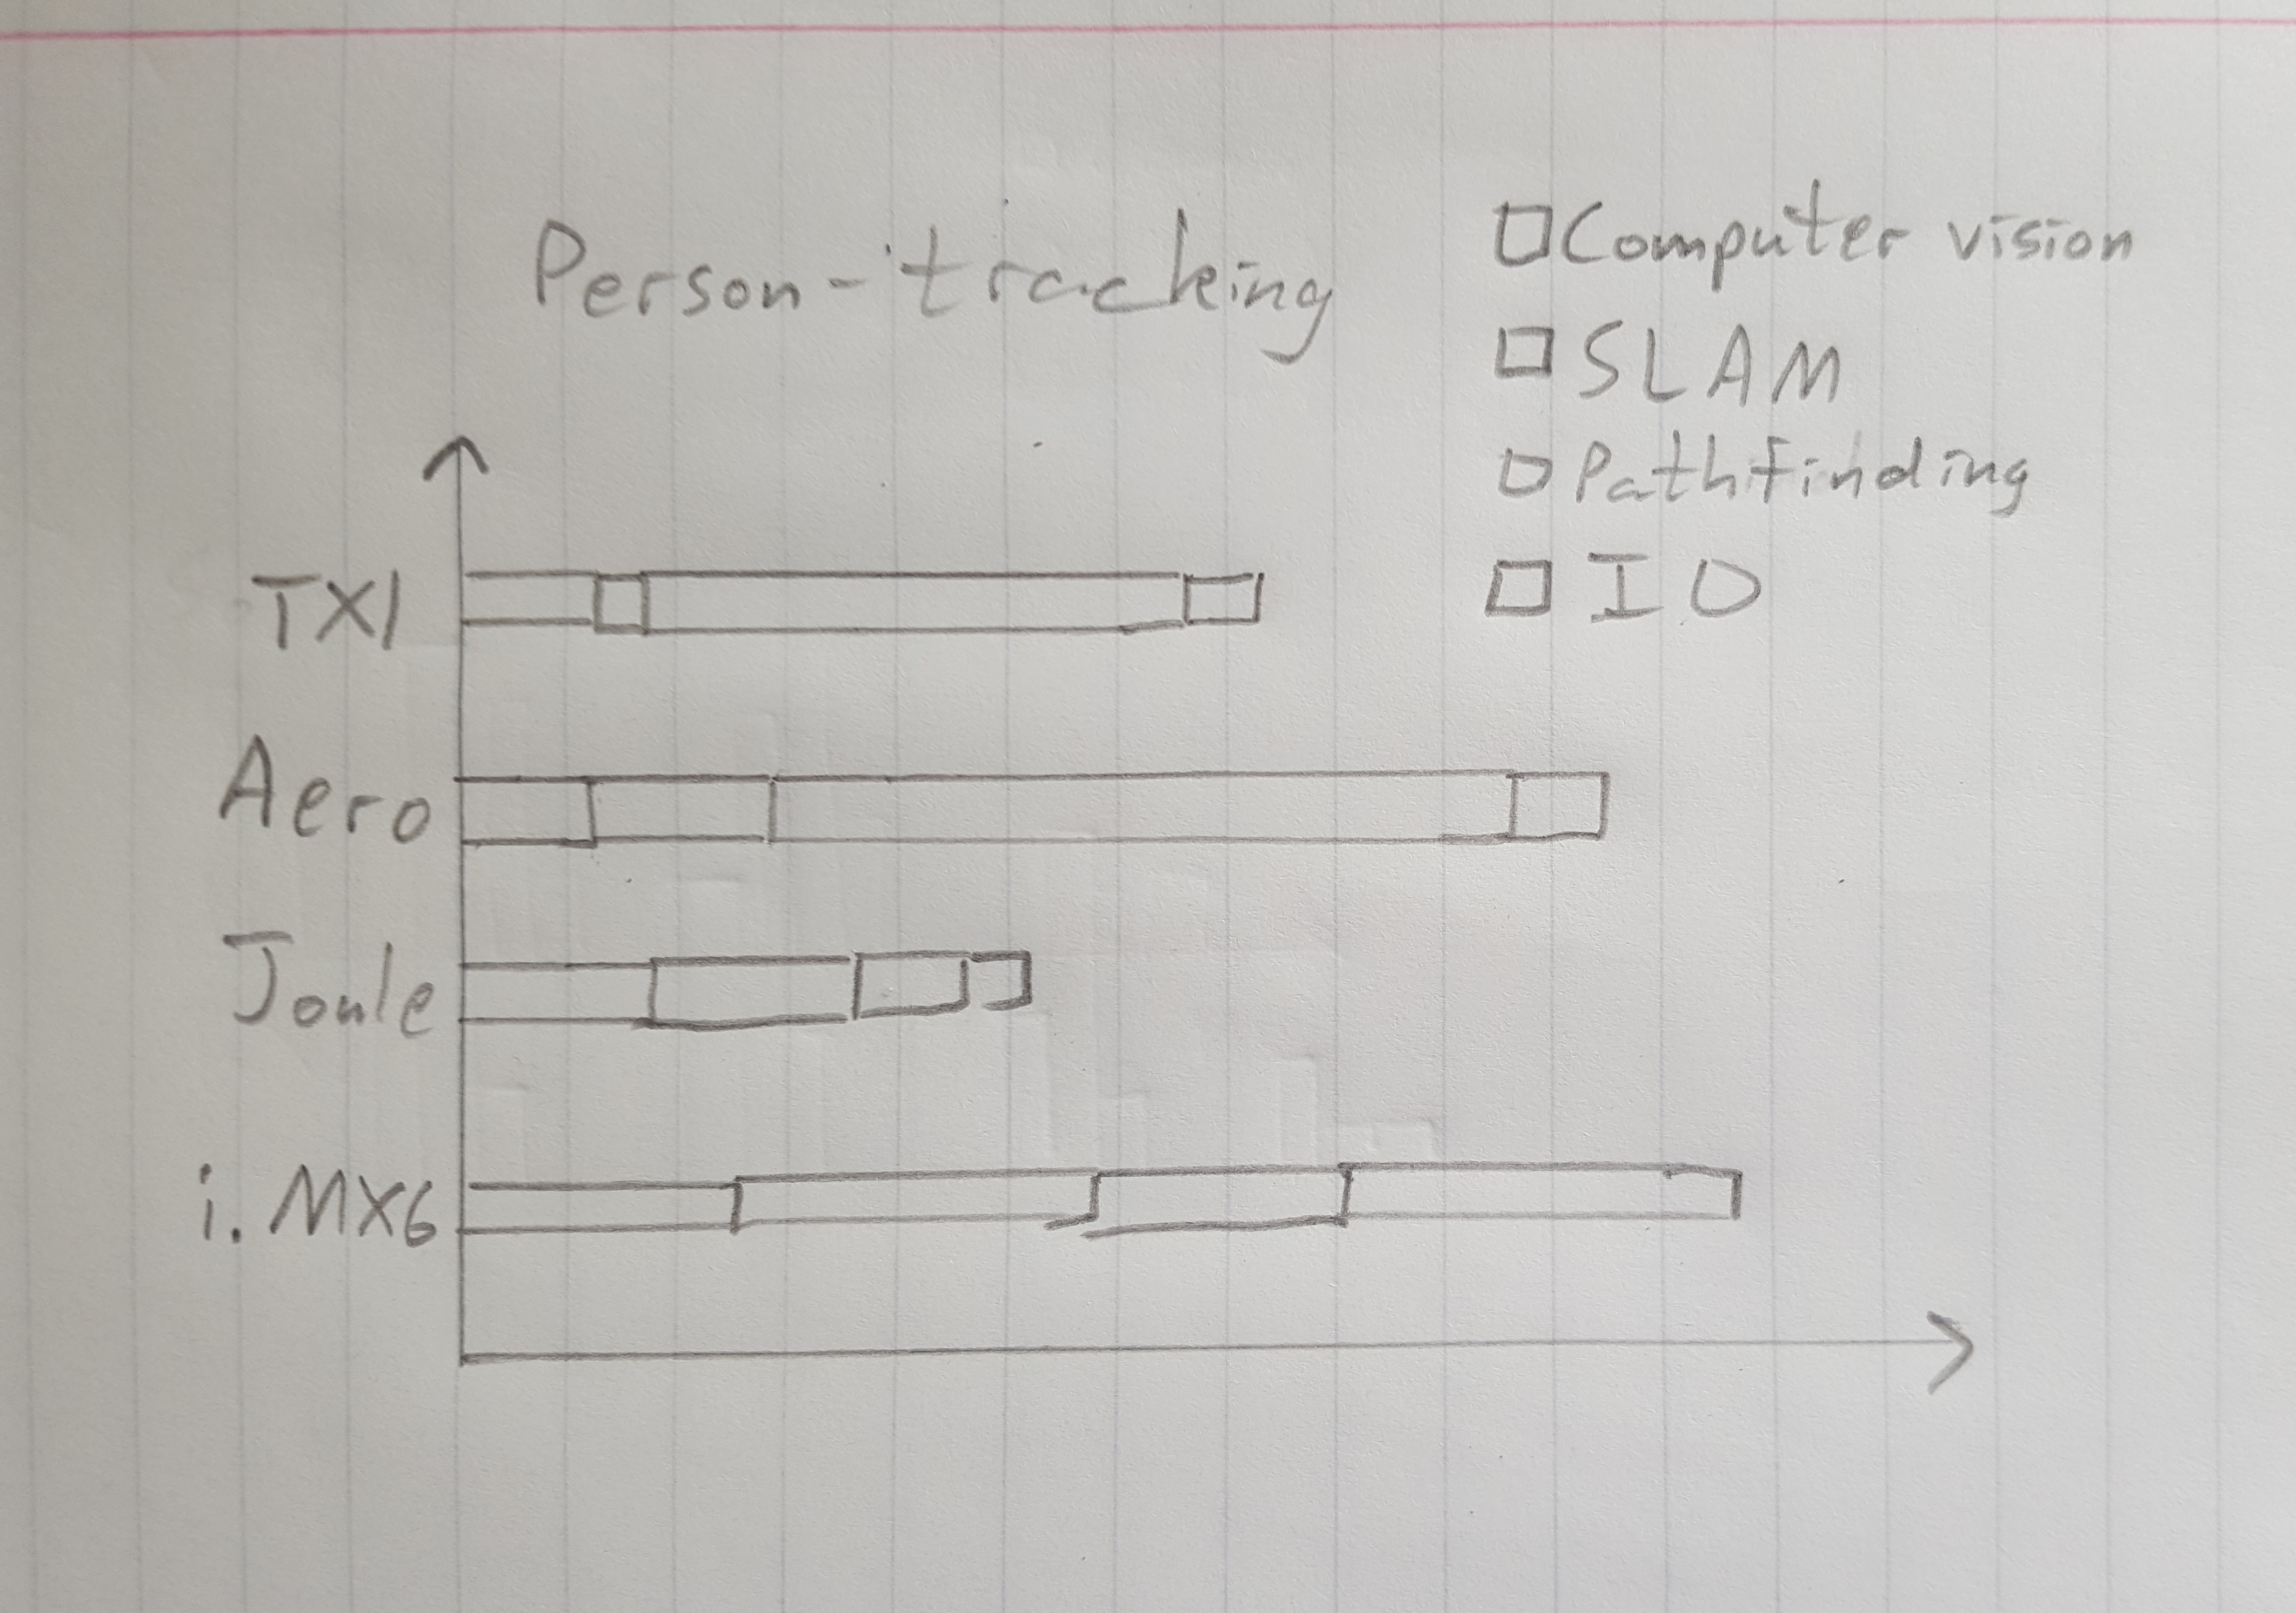
\includegraphics[width=\linewidth]{figs/perf-breakdown}
\caption{Performance breakdown of \textit{Person Tracking} benchmark on AirSim with various companion computers.}
\label{fig:perf-breakdown}
\end{figure}
